% ============================================================
% S2 导学件量产·批1 件1 —— 1.1.1 第1课时 空间向量的概念及线性运算（课时1 导学件·重建版）
% 轮4 成卷·S2 批1｜2026-09-12｜生成链：xelatex main.tex（两遍）→ python render.py（150dpi → png/pageN.png）
%
% 裁决依据（S2就绪报告·主脑裁决回执 2026-09-12）：成卷版课时1 导学件重建为探究点一~四（线性运算域），
%   v11 课1 冻结件（variantF）仅作样式基线不入成卷；A-2 口径：冻结10题计入160满配、导学件例/变式与练习轴互斥照旧。
% 模板承 v11 样张族 `工作区/字替对照-0909/靠齐样张-0910/导学增量/` 六宏＝原样拷贝（L1 冻结参数零改动），
%   局部宏（\pingtou/\liubai/\zhankong）与课时页形制照抄 课时02 首件。
% 章首块＋1.1.1 前衔接六条：装配轮 2026-09-12 已落位（批1值台账 §三.2「留装配轮」登记兑现）——
%   章首三层 \zhangtitle/\jietitle/\xiaojietitle 承 chapterhead.tex 冻结件形（课时层与学习目标维持
%   本件重建版，v11 冻结件仅作样式基线不入成卷）；衔接位「平面向量必会」纯知识点填空六条零题
%   （排产单 §一.1/§2.1＋汇总 §3.1＋定稿A §1.4：不计题、不占衔接 1—29 号段，记「衔接填空①～⑥」，
%   新撰文本全角标点＝义7-1 口径）。chapterhead.tex 同步刷新为启用形（备档副本）。
% 图＝源图位图（禁绘三维，公共规则§5；figs/image2.png 取自 v11 variantF/media/media/ 原图，alt UUID 随带）。
%
% 取材链登记（详见 成卷/导学件/批1值台账.md）：
%   ① 课中探究 例1×4＝讲练件（上）§1.1.1 讲部线性运算域题型段 1.1.1.2-1／1.1.1.3-2／1.1.1.4-3／1.1.1.5-4
%      逐字同文搬运（dump_docx --slice 取证＝工作区/_tmpS2试点0912/讲上-1.1.1全文.txt）；
%      变式1×4＋素养小结×4＝v11 课1 件（variantF/body.tex 探究点一~四）同文承接——重建裁决＝样式宏不动、
%      仅删数量积域内容，线性域件内题面原样保留；与课时01 练习轴同文 4 题（第2/3/6/7题＝练-课-2/3/6/10，
%      A-2 口径下练习轴冻结件本就与 v11 导学件同文）已逐条登记台账，属口径内双印非违规。
%   ② 课前预习 ZSD一/ZSD二＝v11 同文（variantF/body.tex 知识点一/二 含两表，逐字承用）；
%      ZSD三＝讲部 1.1.1-9 共面条目同文化用；判断 5 条＝本轮命制（讲部无判断栏目＝恒命制位，逐题亲算登台账）。
%   ③ 课堂评价恒 5（3 单选＋2 填空、全简单≤例题、填空带提示词＝G5 内构）：
%      第2/3 题＝回收 v11 检测同文（variantF 检测2 k共线／检测4 中点链，均属线性运算域；照裁决回执
%      「可回收 v11 检测降命制量」——回执所载检测2/4/5 按增量样板号＝数量积域三题，属课2 射程，
%      课2 首件已产全命制未回收、不动首件，本批课1 可回收同文号＝线性域两题，命制量 5→3）；
%      第1/4/5 题＝本轮命制，逐题亲算。
%   ④ 与课时01 练习轴 16 题互斥口径：命制位 10 题（判断5＋评价3＋挖空条目不计题）零同文（断言见台账）。
%   ⑤ 句末标点：同文段承源「.」，新命制句用「．」（G8 成卷轮统一清扫，本件不单点改）。
% 编译门：三 0（error＝0／Overfull＝0／Missing character＝0，Underfull 仅计数）——读数见批1值台账。
% ============================================================
\documentclass[fontset=none]{ctexart}
\usepackage{qp-m3} % 换装：六宏→qp-m3 单包（钉后版 md5 7c3930362be8a0a2bdf21bbf8ac16573，两补钉随版）

% ================= 页脚参数宏（qp-headfoot 文件头明示的复用入口，非模块语义改动） =================
\renewcommand{\qpzhangming}{第一章\quad 空间向量与立体几何}
\renewcommand{\qpjianming}{导学件}
\renewcommand{\qpceming}{高中数学\quad 选择性必修第一册(人教B版)} % 换装回钉：qp-m3 默认册名＝选必二，防页脚漂移（试迁规约）

% ================= 局部宏（照抄 v11 导学增量/main.tex 冻结定义；不动公共模块） =================
% 课堂评价组头（XB-02 \zhenhead 同构：\biaoqian 1.3× 标签＋仿宋说明行；恒 5 题说明）
% 局部宏 \pingtou 已由 qp-m3 收编（等值定义），依换装方案§1.4 预删防撞名
% 书写留白＋斜置浅灰水印（导学案正文属性：答案另册→正文留书写位；斜置 25°／black!12）
% 长度 \liubaoh 已由 qp-m3 分配，预删防重复定义
% 局部宏 \liubai 已由 qp-m3 收编（等值定义），依换装方案§1.4 预删防撞名
% 纯书写占位留白（无水印）
% 局部宏 \zhankong 已由 qp-m3 收编（等值定义），依换装方案§1.4 预删防撞名
% 衔接填空条目（装配轮新设局部宏：\tiaomucore 同构——标签「衔接填空①」黑体＋kern8.5pt，非题目不编号）
% 局部宏 \xjtk 已由 qp-m3 收编（等值定义），依换装方案§1.4 预删防撞名

% 纯题版孤行抑制（正装三裁①）：小结②操作/③收束独立段，pure 档整段隐藏，含详解版不受影响
\newcommand{\bindpx}[1]{\ifshowans\bindp{#1}\fi}

% \ov 系答案册 body 局部宏，随值迁入件内补定义（实测 qp-m3 无 \ov，不撞名）
\providecommand{\ov}[1]{\overrightarrow{#1}}

\begin{document}
%成书重装五本跨本连续页码（G7方案B，承M2/M3装配先例）setcounter 注入位
\setcounter{page}{5}

% ============================================================
% 章首块（ZS-01 装饰方块组＋章名＋节名；chapterhead.tex 冻结件形，装配轮落位）
% ============================================================
\zhangtitle{第一章\quad 空间向量与立体几何}
\jietitle{1.1 空间向量及其运算}

% ============================================================
% 1.1.1 前衔接位「衔接：平面向量必会」＝纯知识点填空六条零题（汇总 §3.1／定稿A §1.4；
% 记「衔接填空①～⑥」，不计题数、不占衔接 1—29 号段；逐条与 1.1.1 节内知识点序列对接）
% ============================================================
\keshi{衔接\quad 平面向量必会（1.1.1 前）}
\vspace{1.2mm}
{\fangsong 本块复习必修\allowbreak2平面向量初步的必会知识，为纯知识点填空六条，不计题数、不占衔接题号段（衔接1—29 见 1.2.1 前衔接节）．\par}
\vspace{1.2mm}
\begin{multicols}{2}
\emergencystretch=1em

\xjtk{①}{向量加法法则：\(\overrightarrow{AB}+\overrightarrow{BC}=\)\kongbai{}（三角形法则：首尾相接）；以同一起点的两向量\(\overrightarrow{a}\)，\(\overrightarrow{b}\)为邻边作平行四边形，则\(\overrightarrow{a}+\overrightarrow{b}\)等于以公共起点为起点的\kongbai{}所对应的向量（平行四边形法则）．}

\xjtk{②}{数乘运算及律：\(|\lambda\overrightarrow{a}|=\)\kongbai{}；\((\lambda+\mu)\overrightarrow{a}=\)\kongbai{}，\(\lambda(\overrightarrow{a}+\overrightarrow{b})=\)\kongbai{}（数乘对加法的分配律）．}

\xjtk{③}{共线向量定理：向量\(\overrightarrow{b}\)与非零向量\(\overrightarrow{a}\)共线的充要条件是有且只有\kongbai{}个实数\(\lambda\)，使\(\overrightarrow{b}=\)\kongbai{}.}

\xjtk{④}{平面向量基本定理：如果\(\overrightarrow{e_1}\)，\(\overrightarrow{e_2}\)是同一平面内的两个\kongbai{}向量，那么对于这一平面内的任一向量\(\overrightarrow{a}\)，有且只有一对实数\(\lambda_1\)，\(\lambda_2\)，使\(\overrightarrow{a}=\)\kongbai{}.}

\xjtk{⑤}{数量积定义与运算律：\(\overrightarrow{a}\cdot\overrightarrow{b}=\)\kongbai{}（\(\theta\)为\(\overrightarrow{a}\)与\(\overrightarrow{b}\)的夹角，\(0^{\circ}\leqslant\theta\leqslant180^{\circ}\)）；交换律：\(\overrightarrow{a}\cdot\overrightarrow{b}=\)\kongbai{}；\(\overrightarrow{a}\perp\overrightarrow{b}\Leftrightarrow\)\kongbai{}.}

\xjtk{⑥}{投影数量：设\(\theta\)为非零向量\(\overrightarrow{a}\)与\(\overrightarrow{b}\)的夹角，则\(\overrightarrow{a}\)在\(\overrightarrow{b}\)上的投影数量为\kongbai{}；当\(\theta\)为锐角、直角、钝角时，投影数量的符号依次为\kongbai{}.}

\begin{ansblock}[导-课时01-衔接填空]
% ans:导-课时01-衔接填空
\ansnote{衔接填空}{① \(\ov{AC}\)；对角线。② \(|\lambda||\ov{a}|\)；\(\lambda\ov{a}+\mu\ov{a}\)；\(\lambda\ov{a}+\lambda\ov{b}\)。③ 一；\(\lambda\ov{a}\)。④ 不共线；\(\lambda_{1}\ov{e_{1}}+\lambda_{2}\ov{e_{2}}\)。⑤ \(|\ov{a}||\ov{b}|\cos\theta\)；\(\ov{b}\cdot\ov{a}\)；\(\ov{a}\cdot\ov{b}=0\)。⑥ \(|\ov{a}|\cos\theta\)；正、0、负。}
\end{ansblock}

\end{multicols}

% ============================================================
% 课时页（第1课时；五段闭环，承 v11 导学增量课时页样板形制）
% ============================================================
\xiaojietitle{1.1.1 空间向量及其运算}
\keshi{第1课时\quad 空间向量的概念及线性运算}
\mubiaoline
\mubiaomu{1}{理解空间向量的概念(模、方向、零向量、单位向量、相等向量与相反向量)，会用有向线段表示向量；}
\mubiaomu{2}{掌握空间向量线性运算(加减、数乘)的法则与运算律，理解共线向量、共面向量的充要条件；}
\mubiaomu{3}{会用几何体中的向量作基底表示指定向量，掌握路径分解与系数比较的方法，体会用向量研究几何问题的运算价值.}

\vspace{1.7mm}
\begin{multicols}{2}
\emergencystretch=1em

% ---------- 课前预习（知识导学填空＋诊断分析挂每个知识点之后；ZSD一/二＝v11 同文，ZSD三＝讲部 1.1.1-9 同文） ----------
\huaxing{课}{前}{预}{习}{知识导学\quad 素养初识}

\zsd{一}{空间向量的概念}

\tiaomu{1}{定义：在空间，我们把具有\kongbai{}和\kongbai{}的量叫做空间向量.\zhuzhu{与必修2平面向量初步的定义类比记忆(只多``空间''二字)；零向量方向任意、模为0，是概念题易错点.}}

\tiaomuz{2}{(1)字母表示法：用字母\(\overrightarrow{a},\overrightarrow{b},\overrightarrow{c},\cdots\)表示.}

\bindp (2)几何表示法：用有向线段表示，其\kongbai{}表示空间向量的模.即若向量\(\overrightarrow{a}\)的起点是\(A\)、终点是\(B\)，则向量\(\overrightarrow{a}\)也可记作\(\overrightarrow{AB}\)，其模记为\(| \overrightarrow{AB} |\).\zhuzhu{字母表示与有向线段表示贯穿全章书写，解题前先统一记号；模的记号与绝对值区分，避免混淆.}\tiaomutail

\tiaomu{3}{几类特殊向量(见下表)；规定：\kongbai{}向量与任意向量平行.即对任意向量\(\overrightarrow{a}\)，都有\(\overrightarrow{0}\parallel\overrightarrow{a}\).\zhuzhu{概念辨析高频条目，判定按定义逐条核对；注意共线向量不要求在同一直线上(平行或重合均可)，且零向量与任意向量平行(与共线充要条件衔接).}}

{\setlength{\tabcolsep}{2pt}\arrayrulecolor{gray122}
\vspace{2.55mm}
\noindent\begin{tabular}{!{\vline width 0.8pt}>{\fontsize{10.5pt}{13.9pt}\selectfont\centering\arraybackslash}m{16mm}!{\vline width 0.4pt}>{\fontsize{10.5pt}{13.9pt}\selectfont}m{35.6mm}!{\vline width 0.4pt}>{\fontsize{10.5pt}{13.9pt}\selectfont}m{27.3mm}!{\vline width 0.8pt}}
\thickhline
\makebox[\linewidth]{\textbf{名称}} & \makebox[\linewidth]{\textbf{定义}} & \makebox[\linewidth]{\textbf{表示}} \\[0.45mm]
\hline
\rowreset 零向量\marklines &长度为\kongbai{}的向量叫做零向量\marklines &记作\kongbai{}\marklines \\[\tabrowglue] \hline
\rowreset 单位向量\marklines &模等于\kongbai{}的向量\marklines &用\(e\)表示，\(|e|=1\)\marklines \\[\tabrowglue] \hline
\rowreset 相反向量\marklines &与\(\overrightarrow{a}\)长度相同而方向\kongbai{}的向量\marklines &记作\(-\overrightarrow{a}\)\marklines \\[\tabrowglue] \hline
\rowreset 共线向量或平行向量\marklines &表示若干空间向量的有向线段所在的直线\hspace{0pt plus 1fill}\kongbai{}或\kongbai{}\marklines &记作\(\overrightarrow{a}\parallel\overrightarrow{b}\)\marklines \\[\tabrowglue] \hline
\rowreset 相等向量\marklines &方向相同且\kongbai{}的向量\marklines &记作\(\overrightarrow{a}=\overrightarrow{b}\)\marklines \\[\tabrowglue]
\thickhline
\end{tabular}\par\addvspace{2.8mm}
}

\zhenhead{判断正误(正确的打\gou{},错误的打\cha{})}

\zhentib{(1)}{单位向量都相等．}

\begin{ansblock}[导-课时01-判1]
% ans:导-课时01-判1
\ansitem{(1)}{$\times$}
\end{ansblock}

\zhentib{(2)}{向量\(\overrightarrow{a}\)与\(-\overrightarrow{a}\)互为相反向量，它们的模相等．}

\begin{ansblock}[导-课时01-判2]
% ans:导-课时01-判2
\ansitem{(2)}{\(\surd\)}
\end{ansblock}

\zsd{二}{空间向量的线性运算}

\tiaomu{1}{加法可按\kongbai{}法则或\kongbai{}法则作出；减法\(\overrightarrow{a}-\overrightarrow{b}\)为减向量终点指向被减向量终点；数乘\(\lambda\overrightarrow{a}\)：当\(\lambda>0\)时与\(\overrightarrow{a}\)方向\kongbai{}，当\(\lambda<0\)时方向\kongbai{}，当\(\lambda=0\)时\(\lambda\overrightarrow{a}=\overrightarrow{0}\).\zhuzhu{全章运算的基础，加减、数乘的法则与运算律均与平面向量一致，类比迁移即可；线性组合的运用见共面的充要条件及后续应用.}}

\tiaomu{2}{共线的充要条件：对任意两个空间向量\(\overrightarrow{a},\overrightarrow{b}\)(\(\overrightarrow{b}\neq\overrightarrow{0}\))，\(\overrightarrow{a}\parallel\overrightarrow{b}\)的充要条件是存在\kongbai{} \(\lambda\)，使\(\overrightarrow{a}=\lambda\overrightarrow{b}\).\zhuzhu{证线线平行与求参数存在性的基础工具；易错点：与共面的充要条件混淆------共线用一个实数、共面用有序实数对.}}

{\setlength{\tabcolsep}{3pt}\arrayrulecolor{gray122}
\vspace{2.55mm}
\noindent\begin{tabular}{!{\vline width 0.8pt}>{\fontsize{10.5pt}{13.9pt}\selectfont\centering\arraybackslash}m{10mm}!{\vline width 0.4pt}>{\fontsize{10.5pt}{13.9pt}\selectfont}m{37.6mm}!{\vline width 0.4pt}>{\fontsize{10.5pt}{13.9pt}\selectfont}m{29.2mm}!{\vline width 0.8pt}}
\thickhline
\makebox[\linewidth]{\textbf{运算}} & \makebox[\linewidth]{\textbf{法则要点}} & \makebox[\linewidth]{\textbf{运算律举例}} \\[0.45mm]
\hline
\rowreset 加法\marklines &三角形法则／平行四边形法则(与平面向量一致)\marklines & \(\overrightarrow{a}+\overrightarrow{b}=\overrightarrow{b}+\overrightarrow{a}\)\marklines \\[\tabrowglue] \hline
\rowreset 减法\marklines &减向量终点指向被减向量终点\marklines & \((\overrightarrow{a}+\overrightarrow{b})+\overrightarrow{c}=\overrightarrow{a}+(\overrightarrow{b}+\overrightarrow{c})\)\marklines \\[\tabrowglue] \hline
\rowreset 数乘\marklines &实数\(\lambda\)与向量\(\overrightarrow{a}\)的乘积仍为向量\marklines & \((\lambda+\mu)\overrightarrow{a}=\lambda\overrightarrow{a}+\mu\overrightarrow{a}\)\marklines \\[\tabrowglue] \hline
\rowreset 共线\marklines & \(\overrightarrow{a}\parallel\overrightarrow{b}\)(\(\overrightarrow{b}\neq\overrightarrow{0}\))\marklines & \(\overrightarrow{a}=\lambda\overrightarrow{b}\)\marklines \\[\tabrowglue]
\thickhline
\end{tabular}\par\addvspace{2.8mm}
}

\zhenhead{判断正误(正确的打\gou{},错误的打\cha{})}

\zhentib{(1)}{对任意实数\(\lambda\)和空间向量\(\overrightarrow{a}\)，\(\lambda\overrightarrow{a}\)与\(\overrightarrow{a}\)的方向相同或相反．}

\begin{ansblock}[导-课时01-判3]
% ans:导-课时01-判3
\ansitem{(1)}{$\times$}
\end{ansblock}

\zhentib{(2)}{若\(\overrightarrow{AB}=\overrightarrow{CD}\)，则\(\overrightarrow{AC}=\overrightarrow{BD}\)．}

\begin{ansblock}[导-课时01-判4]
% ans:导-课时01-判4
\ansitem{(2)}{\(\surd\)}
\end{ansblock}

\zsd{三}{空间向量共面的充要条件}

\tiaomu{1}{共面向量：平行于\kongbai{}的向量，叫做共面向量．}

\tiaomu{2}{充要条件：向量\(\overrightarrow{p}\)与\kongbai{}向量\(\overrightarrow{a},\overrightarrow{b}\)共面的充要条件是存在唯一的有序实数对\((x,y)\)，使\(\overrightarrow{p}=x\overrightarrow{a}+y\overrightarrow{b}\).\zhuzhu{证四点共面、线共面的标准工具；易错点：定理前提是a、b不共线，此前提不可漏，且实数对存在唯一.}}

\begin{ansblock}[导-课时01-预习填空]
% ans:导-课时01-预习填空
\ansnote{预习填空}{知识点一：大小、方向；长度；零；0、\(\overrightarrow{0}\)、1、相反、平行、重合、模相等。知识点二：三角形、平行四边形；相同；相反；唯一。知识点三：同一平面；不共线。}
\end{ansblock}

\zhenhead{判断正误(正确的打\gou{},错误的打\cha{})}

\zhentib{(1)}{若\(\overrightarrow{a}\)，\(\overrightarrow{b}\)不共线，则对空间任意一个向量\(\overrightarrow{p}\)，都存在有序实数对\((x,y)\)，使\(\overrightarrow{p}=x\overrightarrow{a}+y\overrightarrow{b}\)．}

\begin{ansblock}[导-课时01-判5]
% ans:导-课时01-判5
\ansitem{(1)}{$\times$}
\end{ansblock}

\liubai[9mm]{此处书写}

% ---------- 课中探究（探究点一~四；例1×4＝讲部线性域同文搬运，变式1×4＋小结＝v11 课1 件线性域承用） ----------
\huaxing{课}{中}{探}{究}{考点探究\quad 素养小结}

\tjdnr{一}{空间向量的概念辨析}{例\textbf{1}}{简单(知识点一)}{下列说法正确的是\nobreak(\kongwei)}

\bindopt {\fontsize{10.5pt}{19pt}\selectfont A．若\(| \overrightarrow{a} | = | \overrightarrow{b} |\)，则\nobreak\(\overrightarrow{a} = \overrightarrow{b}\)或\(\overrightarrow{a} = - \overrightarrow{b}\)；\par}

\bindopt {\fontsize{10.5pt}{19pt}\selectfont B．若\(\overrightarrow{a},\overrightarrow{b}\)为相反向量，则\nobreak\(\overrightarrow{a} + \overrightarrow{b} = \overrightarrow{0}\)；\par}

\bindopt {\fontsize{10.5pt}{19pt}\selectfont C．零向量是没有方向的向量；\par}

\bindopt {\fontsize{10.5pt}{19pt}\selectfont D．若\(\overrightarrow{a},\overrightarrow{b}\)是两个单位向量，则\nobreak\(\overrightarrow{a} = \overrightarrow{b}\)\par}

\liubai[6mm]{解答书写区}

\begin{ansblock}[导-课时01-探1-例1]
% ans:导-课时01-探1-例1
\ansnote{例1}{B}
\end{ansblock}

\liB{变式\textbf{1}}{简单(知识点一)}{}{下列说法错误的是\nobreak(\kongwei)}

\bindopt {\fontsize{10.5pt}{19pt}\selectfont A．零向量与任意向量都平行；\par}

\bindopt {\fontsize{10.5pt}{19pt}\selectfont B．若\(|\overrightarrow{a}|=0\)，则\nobreak\(\overrightarrow{a}=\overrightarrow{0}\)；\par}

\bindopt {\fontsize{10.5pt}{19pt}\selectfont C．若\(\overrightarrow{a}=\overrightarrow{b}\)，则\nobreak\(|\overrightarrow{a}|=|\overrightarrow{b}|\)；\par}

\bindopt {\fontsize{10.5pt}{19pt}\selectfont D．若\(\overrightarrow{a}\parallel\overrightarrow{b}\)，则\nobreak\(|\overrightarrow{a}|=|\overrightarrow{b}|\)\par}

\begin{ansblock}[导-课时01-探1-变式1]
% ans:导-课时01-探1-变式1
\ansnote{变式1}{D}
\end{ansblock}

\xiaojie{①识别：题干围绕模、方向、零向量、单位向量、相等向量与相反向量罗列说法要求辨误时，判归本题型.}

\bindpx {\kaishu ②操作：对照定义逐条核验，存疑条目用反例否定.}

\bindpx {\kaishu ③收束：排除错误项定答案，忌凭直觉误选.}

\tjdnr{二}{空间向量的线性运算}{例\textbf{1}}{简单(知识点二)}{在直三棱柱\(ABC\text{-}\penalty100 A_{1}B_{1}C_{1}\)中，若\(\overrightarrow{CA} = \overrightarrow{a},\overrightarrow{CB} = \overrightarrow{b},\overrightarrow{CC_{1}} = \overrightarrow{c},\)，则\nobreak\(\overrightarrow{A_{1}B}\)=\kongbai{}.(用\(\overrightarrow{a},\overrightarrow{b},\overrightarrow{c}\)表示)}

\liubai[6mm]{解答书写区}

\begin{ansblock}[导-课时01-探2-例1]
% ans:导-课时01-探2-例1
\ansnote{例1}{\(\overrightarrow{b}-\overrightarrow{a}-\overrightarrow{c}\)}
\end{ansblock}

\liB{变式\textbf{1}}{简单(知识点二)}{}{在平行六面体\(ABCD\text{-}\penalty100 A_1B_1C_1D_1\)中，\(\overrightarrow{AB}=\overrightarrow{a}\)，\(\overrightarrow{AD}=\overrightarrow{b}\)，\(\overrightarrow{AA_1}=\overrightarrow{c}\)，则\nobreak\(\overrightarrow{D_1B}=\)\kongbai{}.(用\(\overrightarrow{a}\)，\(\overrightarrow{b}\)，\(\overrightarrow{c}\)表示)}

\begin{ansblock}[导-课时01-探2-变式1]
% ans:导-课时01-探2-变式1
\ansnote{变式1}{\(\overrightarrow{a}-\overrightarrow{b}-\overrightarrow{c}\)}
\end{ansblock}

\xiaojie{①识别：在几何体中给出若干已知向量、要求表示指定向量时，判归本题型.}

\bindpx {\kaishu ②操作：为目标向量选一条首尾相接的路径写出加减链，再把链中各段用相等或共线的已知向量替换，最后合并化简得表达式.}

\bindpx {\kaishu ③收束：复查每段方向与起讫点，防抄错向量.}

\tjdnr{三}{用基底表示向量}{例\textbf{1}}{简单(知识点二)}{}

\noindent\begin{minipage}[t]{46.368mm}\raggedright 已知正方体\emph{ABCD}-\emph{A\textsubscript{1}B\textsubscript{1}C\textsubscript{1}D\textsubscript{1}}中，\(\overrightarrow{A_{1}E}\)=\(\frac{1}{4}\) \(\overrightarrow{A_{1}C_{1}}\)，若\(\overrightarrow{AE} =\)\emph{x}\(\overrightarrow{AA_{1}}\)+\emph{y}(\(\overrightarrow{AB}\)+\(\overrightarrow{AD}\))，则\emph{x}\nobreak=\kongbai{}，\emph{y}\nobreak=\kongbai{}.\end{minipage}\hspace{0.925mm}\begin{minipage}[t]{32.000mm}\centering\raisebox{\dimexpr-\height+3.545mm\relax}[\dimexpr3.545mm\relax][\dimexpr\height-3.545mm\relax]{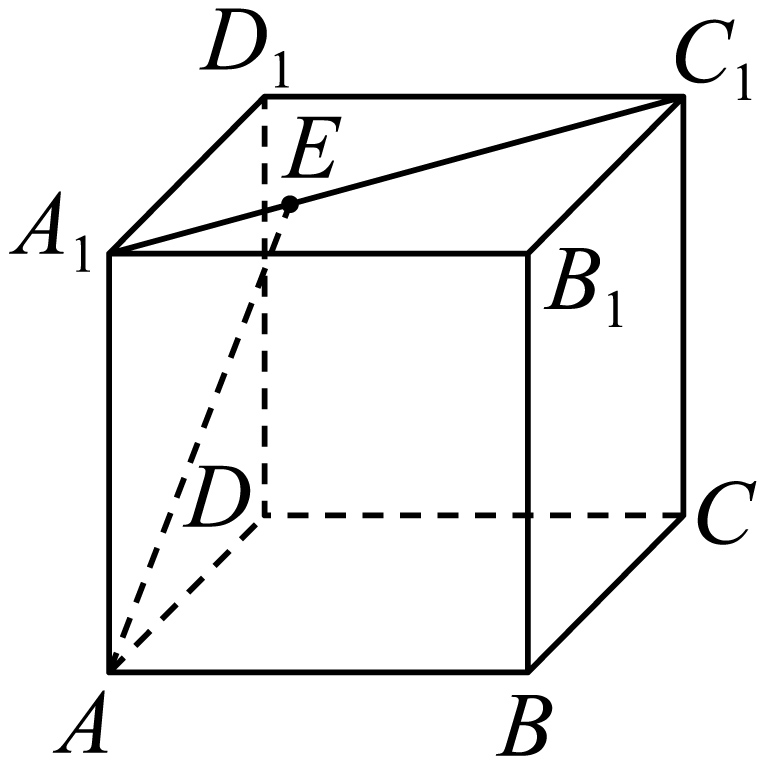
\includegraphics[width=32.000mm,alt={@@@b0b55c9f-4634-4bba-b096-bc6dd0cf7747}]{figs/image2.png}}\end{minipage}\par

\begin{ansblock}[导-课时01-探3-例1]
% ans:导-课时01-探3-例1
\ansnote{例1}{\(x=1\)，\(y=\dfrac{1}{4}\)}
\end{ansblock}

\liB{变式\textbf{1}}{简单(知识点二)}{}{在平行六面体\(ABCD\text{-}\penalty100 A_1B_1C_1D_1\)中，点\(E\)在\(A_1C_1\)上，且\(\overrightarrow{A_1E}=\frac{1}{2}\overrightarrow{A_1C_1}\)，若\(\overrightarrow{AE}=x\overrightarrow{AA_1}+y(\overrightarrow{AB}+\overrightarrow{AD})\)，则\nobreak\(x=\)\kongbai{}，\(y=\)\kongbai{}.}

\begin{ansblock}[导-课时01-探3-变式1]
% ans:导-课时01-探3-变式1
\ansnote{变式1}{\(x=1\)，\(y=\dfrac{1}{2}\)}
\end{ansblock}

\xiaojie{①识别：指定三个不共面的向量作基底、要求把目标向量写成基底向量的线性组合并求系数时，判归本题型.}

\bindpx {\kaishu ②操作：先把目标向量沿几何路径分解为基底向量的和，再把各段按比例关系代入基底.}

\bindpx {\kaishu ③收束：比较等式两边系数求出待定值，防漏写中间段.}

\tjdnr{四}{共面向量的判定}{例\textbf{1}}{简单(知识点三)}{有下列说法:}

\bindopt ①若\(\overrightarrow{p} = x\overrightarrow{a} + y\overrightarrow{b}\)，则\nobreak\(\overrightarrow{p}\)与\(\overrightarrow{a}\)，\(\overrightarrow{b}\)共面；②若\(\overrightarrow{p}\)与\(\overrightarrow{a}\)，\(\overrightarrow{b}\)共面，则\nobreak\(\overrightarrow{p}\)=\emph{x}\(\overrightarrow{a}\)+\emph{y}\(\overrightarrow{b}\)；③若\(\overrightarrow{MP}\)=\emph{x}\(\overrightarrow{MA}\)+\emph{y}\(\overrightarrow{MB}\)，则\emph{P}，\emph{M}，\emph{A}，\emph{B}共面；④若\emph{P}，\emph{M}，\emph{A}，\emph{B}共面，则\nobreak\(\overrightarrow{MP}\)=\emph{x}\(\overrightarrow{MA}\)+\emph{y}\(\overrightarrow{MB}\).其中正确的是\nobreak(\kongwei)

\bindopt {\fontsize{10.5pt}{19pt}\selectfont \makebox[\dimexpr0.5\linewidth-1em\relax][l]{A．①②③④；}\makebox[\dimexpr0.5\linewidth-1em\relax][l]{B．①③④；}\par}

\bindopt {\fontsize{10.5pt}{19pt}\selectfont \makebox[\dimexpr0.5\linewidth-1em\relax][l]{C．①③；}\makebox[\dimexpr0.5\linewidth-1em\relax][l]{D．②④}\par}

\liubai[6mm]{解答书写区}

\begin{ansblock}[导-课时01-探4-例1]
% ans:导-课时01-探4-例1
\ansnote{例1}{C（①③）}
\end{ansblock}

\liB{变式\textbf{1}}{简单(知识点三)}{}{已知\(\overrightarrow{MP}=3\overrightarrow{MA}-2\overrightarrow{MB}\)，判断\(P\)，\(M\)，\(A\)，\(B\)四点是否共面，并说明理由.}

\begin{ansblock}[导-课时01-探4-变式1]
% ans:导-课时01-探4-变式1
\ansnote{变式1}{共面}
\end{ansblock}

\xiaojie{①识别：题干给出p=xa+yb或MP=xMA+yMB一类线性表示与“共面”结论的互推说法判断时，判归本题型.}

\bindpx {\kaishu ②操作：核对充要条件的前提(两向量不共线或三点不共线)是否齐备，再对缺前提的说法举共线反例排除.}

\bindpx {\kaishu ③收束：最后汇总正确序号定选项.}

% ---------- 课堂评价（恒 5 题＝3 单选＋2 填空；全简单≤例题；提示词形制；第2/3题回收 v11 检测同文，第1/4/5题本轮命制——逐题亲算登批1值台账） ----------
\begin{ketang}{本组共5题，1—3为单选，4—5为填空．}

\jiancestem{{\fontsize{11.4pt}{14pt}\selectfont\heihao {\numboldjian 1}．}\hspace{4.1mm}\tieside{简单(知识点一)}\hspace{2.2mm}下列说法正确的是(\kongwei)}

\bindopt {\fontsize{10.5pt}{21pt}\selectfont A．平行向量一定是相等向量；\par}

\bindopt {\fontsize{10.5pt}{21pt}\selectfont B．共线向量一定是方向相同的向量；\par}

\bindopt {\fontsize{10.5pt}{21pt}\selectfont C．相等向量的方向一定相同；\par}

\bindopt {\fontsize{10.5pt}{21pt}\selectfont D．方向相同的向量一定是相等向量\par}

\begin{ansblock}[导-课时01-评1]
% ans:导-课时01-评1
\ansitem{1}{C}
\end{ansblock}

\jiancestem{{\fontsize{11.4pt}{14pt}\selectfont\heihao {\numboldjian 2}．}\hspace{4.1mm}\tieside{简单(知识点二)}\hspace{2.2mm}设\(\overrightarrow{e_1}\)，\(\overrightarrow{e_2}\)不共线，\(\overrightarrow{a}=2\overrightarrow{e_1}+\overrightarrow{e_2}\)，\(\overrightarrow{b}=4\overrightarrow{e_1}+k\overrightarrow{e_2}\)，若\(\overrightarrow{a}\parallel\overrightarrow{b}\)，则\nobreak\(k=\)(\kongwei)}

\bindopt {\fontsize{10.5pt}{21pt}\selectfont \makebox[\dimexpr0.25\linewidth-0.5em\relax][l]{A．\(\frac{1}{2}\)；}\makebox[\dimexpr0.25\linewidth-0.5em\relax][l]{B．\(2\)；}\makebox[\dimexpr0.25\linewidth-0.5em\relax][l]{C．\(-\frac{1}{2}\)；}\makebox[\dimexpr0.25\linewidth-0.5em\relax][l]{D．\(3\)}\par}

\begin{ansblock}[导-课时01-评2]
% ans:导-课时01-评2
\ansitem{2}{B（2）}
\end{ansblock}

\jiancestem{{\fontsize{11.4pt}{14pt}\selectfont\heihao {\numboldjian 3}．}\hspace{4.1mm}\tieside{简单(知识点二)}\hspace{2.2mm}在空间四边形\(ABCD\)中，\(E\)，\(F\)分别为\(AB\)，\(CD\)的中点，则\nobreak\(\frac{1}{2}(\overrightarrow{AD}+\overrightarrow{BC})=\)(\kongwei)}

\bindopt {\fontsize{10.5pt}{21pt}\selectfont \makebox[\dimexpr0.25\linewidth-0.5em\relax][l]{A．\(2\overrightarrow{EF}\)；}\makebox[\dimexpr0.25\linewidth-0.5em\relax][l]{B．\(-\overrightarrow{EF}\)；}\makebox[\dimexpr0.25\linewidth-0.5em\relax][l]{C．\(\overrightarrow{FE}\)；}\makebox[\dimexpr0.25\linewidth-0.5em\relax][l]{D．\(\overrightarrow{EF}\)}\par}

\begin{ansblock}[导-课时01-评3]
% ans:导-课时01-评3
\ansitem{3}{D（\(\overrightarrow{EF}\)）}
\end{ansblock}

\jiancestem{{\fontsize{11.4pt}{14pt}\selectfont\heihao {\numboldjian 4}．}\hspace{4.1mm}\tieside{简单(知识点二)}\hspace{2.2mm}在四面体\(ABCD\)中，\(\overrightarrow{DA}=\overrightarrow{a}\)，\(\overrightarrow{DB}=\overrightarrow{b}\)，\(\overrightarrow{DC}=\overrightarrow{c}\)，\(M\)为\(BC\)的中点，则\nobreak\(\overrightarrow{AM}=\)\kongbai{}（用\(\overrightarrow{a},\overrightarrow{b},\overrightarrow{c}\)表示）．{\zhushi{(提示：\(\overrightarrow{AM}=\overrightarrow{DM}-\overrightarrow{DA}\)，且\(\overrightarrow{DM}=\frac{1}{2}(\overrightarrow{DB}+\overrightarrow{DC})\))}}}

\begin{ansblock}[导-课时01-评4]
% ans:导-课时01-评4
\ansitem{4}{\(-\overrightarrow{a}+\dfrac{1}{2}\overrightarrow{b}+\dfrac{1}{2}\overrightarrow{c}\)}
\end{ansblock}

\jiancestem{{\fontsize{11.4pt}{14pt}\selectfont\heihao {\numboldjian 5}．}\hspace{4.1mm}\tieside{简单(知识点三)}\hspace{2.2mm}已知\(\overrightarrow{a}\)，\(\overrightarrow{b}\)，\(\overrightarrow{c}\)是两两不平行的空间向量，则其中共面向量的对数为\kongbai{}．{\zhushi{(提示：任意两个空间向量都可以平移到同一个平面内，即``两向量必共面'')}}}

\begin{ansblock}[导-课时01-评5]
% ans:导-课时01-评5
\ansitem{5}{3}
\end{ansblock}

\end{ketang}

\end{multicols}

\tailfill
\end{document}
